\section{Лекция 2. Конечные автоматы.}

\begin{Def} \label{eq:FA}
    \textbf{\text{Конечный автомат }} $\mathcal{A}$ --- устройство, описываемое набором \\$\langle Q$, $\Sigma$, $q_0$, $\delta$, $F \rangle$:
    \begin{enumerate}
        \item {\bfseries\itshape{Q}} - конечное множество состояний автомата;
        \item $\boldsymbol{\Sigma}$ - алфавит, слова над которым обрабатывает автомат;
        \item $\boldsymbol{q_0}$ - начальное состояние автомата;
        \item $\boldsymbol{\delta}$ : $Q \times (\Sigma\cup\{\varepsilon\} ) \rightarrow 2^{Q}$ - функция переходов
        \item $\boldsymbol{F} \subset \boldsymbol{Q}$ - множество принимающих состояний.
    \end{enumerate}
\end{Def}

Напомним, что $2^Q$ - множество всех подмножеств Q (булеан). Запись $f: A \rightarrow B $ означает, что функция определена на всех элементах множества $A$. Мы считаем, что если $\delta (q,\sigma) = \emptyset$, то переход из состояния $q$  по символу $\sigma \in \Sigma \cup \{ \varepsilon \}$ не  определен.


\textbf{Пример 1. Диаграмма Мура}
\begin{center}
    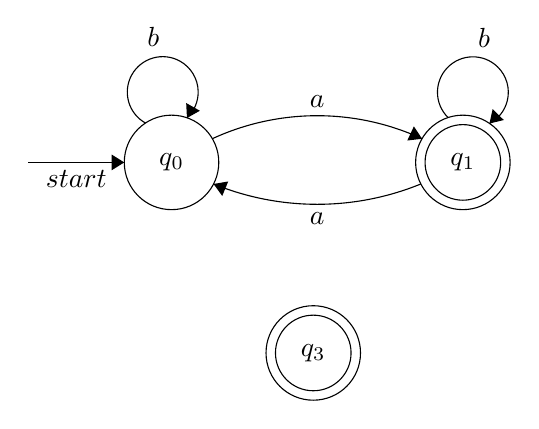
\begin{tikzpicture}[scale=0.2]
        \tikzstyle{every node}+=[inner sep=0pt]
        \draw [black] (16.1,-27) circle (3);
        \draw (16.1,-27) node {$q_0$};
        \draw [black] (34.6,-27) circle (3);
        \draw (34.6,-27) node {$q_1$};
        \draw [black] (34.6,-27) circle (2.4);
        \draw [black] (25.1,-39.1) circle (3);
        \draw (25.1,-39.1) node {$q_3$};
        \draw [black] (25.1,-39.1) circle (2.4);
        \draw [black] (7,-27) -- (13.1,-27);
        \fill [black] (13.1,-27) -- (12.3,-26.5) -- (12.3,-27.5);
        \draw (10.05,-27.5) node [below] {$start$};
        \draw [black] (18.69,-25.495) arc (114.75276:65.24724:15.906);
        \fill [black] (32.01,-25.5) -- (31.49,-24.71) -- (31.07,-25.61);
        \draw (25.35,-23.53) node [above] {$a$};
        \draw [black] (31.934,-28.368) arc (-67.77817:-112.22183:17.409);
        \fill [black] (18.77,-28.37) -- (19.32,-29.13) -- (19.7,-28.21);
        \draw (25.35,-30.16) node [below] {$a$};
        \draw [black] (14.455,-24.505) arc (241.12502:-46.87498:2.25);
        \draw (14.95,-19.7) node [above] {$b$};
        \fill [black] (17.08,-24.18) -- (17.9,-23.72) -- (17.03,-23.23);
        \draw [black] (33.67,-24.16) arc (225.8699:-62.1301:2.25);
        \draw (35.95,-19.71) node [above] {$b$};
        \fill [black] (36.29,-24.53) -- (37.2,-24.31) -- (36.49,-23.61);
    \end{tikzpicture}
\end{center}

Автоматы удобно представлять не набором множеств, а автоматом (Диаграмма Мура).

Каждое состояние обозначаем отдельным кругом (внутри впишем название состояния). Двойной кружок - принимающее состояние. Входная стрелка у начального состояние. Определим переходы: переход из состояния из $q_0$ в $q_1$ по символу a обозначим стрелкой. Впишем обратный переход. Петля будет вести из данного состояния в него же.

Автомат принимает слово с точки зрения графов - есть путь из начального состояния в принимающее, если автомат ДКА, то это путь определенном однозначно, для НКА не обязательно путь должен быть определен однозначно, и вдоль этого пути написано наше слово, принадлежность которого мы проверяем.

Распишем формально наш автомат.
\begin{enumerate}
    \item {\bfseries\itshape{Q}} - \{$q_0, q_1, q_3$\}
    \item $\boldsymbol{\Sigma}$ - \{$a,b$\};
    \item $\boldsymbol{q_0}$ -$q_0$
    \item $\boldsymbol{\delta}$ : $(\{q_0,b,q_0\}, \{q_0,a,q_1\},\{q_1,b,q_1\},\{q_1,a,q_0\})$
    \item $\boldsymbol{F} \subset \boldsymbol{Q}$ - \{$q_1,q_3$\}
\end{enumerate}

\textbf{Конфигурация автомата}
Конфигурацией конечного автомата называется $$\mathcal{A} = \langle Q, \Sigma, q_s, F, \delta\rangle$$ называется элемент множества $Conf(\mathcal{A}) = Q\times \Sigma^*$

\textbf{Отношение достижимости}
Зададим следующее отношение $\vdash^* \ \subset \ Conf(\mathcal{A})^2$:
\begin{itemize}
    \item $\forall q \in Q, w \in \Sigma^*: (q, w) \vdash^* (q, w)$
    \item $(q_1, xay) \vdash^* (q_2, ay) \vee (q_2, a, q_3) \in \delta \Rightarrow (q_1, xay) \vdash^* (q_3, y).$
\end{itemize}
Если $\forall x: (p, wx) \vdash^* (q, x)$, то будем писать $p \xrightarrow{w} q$.


\textbf{Слово принимаемое автоматом}
Будем говорить что слово $w$ принимается автоматом если для некоторого $q_f \in F$ верно $(q_s, w) \vdash^* (q_f, \varepsilon)$. Иначе говоря, если <<идя по стрелочкам>> в автомате по этому слову и правильно выбирая путь можно дойти до финального состояния.

\textbf{Язык принимаемый автоматом}
Язык автомата $\mathcal{A}$ --- это множество $L(\mathcal{A})$ всех слов принимаемых автоматом. Будем говорить, что конечный автомат принимает язык $B$ если $B = L(\mathcal{
        A})$. Будем говорить что два автомата $\mathcal{A}, \mathcal{B}$ эквивалентны, если $L(\mathcal{A})=L(\mathcal{B})$.

\textbf{Автоматный язык}
Язык называется автоматным если он принимается каким-либо конечным автоматом.

\textbf{Теорема Клини}
Класс автоматных языков и класс регулярных языков совпадают.

\textbf{Построение НКА и РВ}
Пусть $\Sigma = \{a, b\}$. Постройте НКА и РВ которые принимают язык $$ L = \{w\ | \ w[|w|-2]=b\} $$

Для начала построим РВ. Рассмотрим $(a+b)^*b(a+b)^2$. Любое слово $w$, порожденное этим РВ имеет вид $w = \alpha b \beta, |\beta| = 2$, а соответственно $w \in L$. С другой стороны любое слово $v \in L$, $v = \alpha b \beta, |\beta| = 2$, а значит порождается РВ.\\
Теперь построим НКА:
\begin{center}
    \begin{tikzpicture}[->,shorten >=1pt,auto,node distance=2.8cm]
        \node[initial,state]      (A)                  {$q_1$};
        \node[state]              (B) [right of=A]     {$q_2$};
        \node[state]              (C) [right of=B]     {$q_3$};
        \node[accepting, state]   (D) [right of=C]     {$q_4$};

        \path (A) edge [loop above] node {a} (A)
        edge [loop below] node {b} (A)
        edge              node {b} (B)
        (B) edge [bend right] node {b} (C)
        edge [bend left]  node {a} (C)
        (C) edge [bend right] node {b} (D)
        edge [bend left]  node {a} (D);
    \end{tikzpicture}
\end{center}
Как мы уже поняли язык $L$ это язык таких слов $w$, что $w = \alpha b \beta, |\beta| = 2$. Из построения видно, что $q_1 \xrightarrow{\alpha} q_1, q_1 \xrightarrow{b} q_2, q_2 \xrightarrow{\beta} q_4$. А это означает, что $q_1 \xrightarrow{\alpha b \beta} q_4$.
Теперь распишем определение.
Если $\forall x: (p, wx) \vdash^* (q, x)$, то будем писать $p \xrightarrow{w} q$.
Подставим $\varepsilon$ вместо $x$ и получим
$(q_1, w) \vdash^* (q_4, \varepsilon)$, что означает что автомат принимает все слова из $L$. \\
Покажем что любое слово принятое автоматом принадлежит $L$. Пусть автомат принял слово $w$, тогда $\exists \alpha, \gamma, \beta: q_1 \xrightarrow{\alpha} q_1 \xrightarrow{\gamma} q_2 \xrightarrow{\beta} q_4$. Из конструкции автомата видно что $\alpha \in (a+b)^*, \beta \in  (a+b)^2, \gamma = b$, а значит принятое слово лежит в языке задаваемым РВ $(a+b)^*b(a+b)^2$.

\textbf{Построение НКА}
Пусть $\Sigma = \{a, b\}$. Постройте НКА который принимает язык $$ L = \{w\ | \ |w|_a + 2|w|_b = 0 \mod 5\} $$

Рассмотрим автомат:
\begin{center}
    \begin{tikzpicture}[->,shorten >=1pt,auto,node distance=2.8cm]
        \node[]                       (dummy)                       {};
        \node[initial,accepting,state](A) [above left of=dummy]     {$[0]$};
        \node[state]                  (B) [above of=dummy]          {$[1]$};
        \node[state]                  (C) [above right of=dummy]    {$[2]$};
        \node[state]                  (D) [below right of=dummy]    {$[3]$};
        \node[state]                  (E) [below left of=dummy]     {$[4]$};

        \path (A) edge [bend left] node {a}        (B)
        edge             node [swap] {b} (C)
        (B) edge [bend left] node {a}        (C)
        edge             node [swap] {b} (D)
        (C) edge [bend left] node {a}        (D)
        edge             node [swap] {b} (E)
        (D) edge [bend left] node {a}        (E)
        edge             node [swap] {b} (A)
        (E) edge [bend left] node {a}        (A)
        edge             node [swap] {b} (B);
    \end{tikzpicture}
\end{center}
Будем доказывать по индукции следующее утверждение: прочитав слово $w : |w|_a + 2|w|_b = i \mod 5$ автомат находится в состоянии $[i]$, формально говоря $[0] \xrightarrow{w} [i]$.
\begin{itemize}
    \item База: прочитав слово $\varepsilon$ автомат находится в состоянии $[0]$.
    \item Предположение: пусть утверждение верно для всех слов длины $n$.
    \item Шаг: Рассмотрим без ограничения общности слово $w:|w|=n+1$. Слово $w$ можно представить как $w=\alpha\beta, |\alpha| = n, |\beta| = 1$. По предположению индукции $[0] \xrightarrow{\alpha} [j], |\alpha|_a + 2|\alpha|_b = j \mod 5$. Но как можно заметить из построения автомата $[j] \xrightarrow{a} [j+1 \mod 5]$, $[j] \xrightarrow{b} [j+2 \mod 5]$. Утверждение доказанно.
\end{itemize}

\subsection{Алгоритм построеня ДКА по РВ}
На прошлой лекции мы убедились, что РВ порождает все регулярные языки (по определению), далее мы познакомились с ДКА. Оказывается, что языки, распознаваемые НКА и ДКА и языки, задаваемые РВ "--- это один и тот же класс языков (Регулярные языки). Далее мы не будем рассматривать РВ, в которых етсь пустое множество.

Давайте занумеруем все позиции в РВ (например, как в \eqref{eq:R}) и допишем два дополнительных символа: маркер начала слова $\rhd$ и маркер конца слова $\lhd$. Нам будет интересно из какой позиции порождён тот или иной символ слова. Таких позиций может быть несколько. Наш алгоритм будет запоминать их все. Для этого определим вспомогательное множество $FollowPos$ для каждой позиции:
\begin{Def}
    $FollowPos(i \sigma)$ - {i $\sigma'$: i $\sigma'$ может идти в слове после $i\sigma$}
\end{Def}


Будем строить ДКА по следующему РВ с помощью вспомогательного множества --- $FollowPos$
\begin{equation}\label{eq:R}
    R = \underset{0}{\rhd}(\underset{1}{a}\underset{2}{a}|\underset{3}{b})^{*}\underset{4}{b}(\underset{5}{a}|\underset{6}{b})^{*}\underset{7}{a}\underset{8}{\lhd}.
\end{equation}

Чтобы вычислить множество $FollowPos$, нам понадобится представление формулы \ref{eq:R} в виде графа, который называется синтаксическим деревом:


\begin{figure}[h!tp]
    \centering
    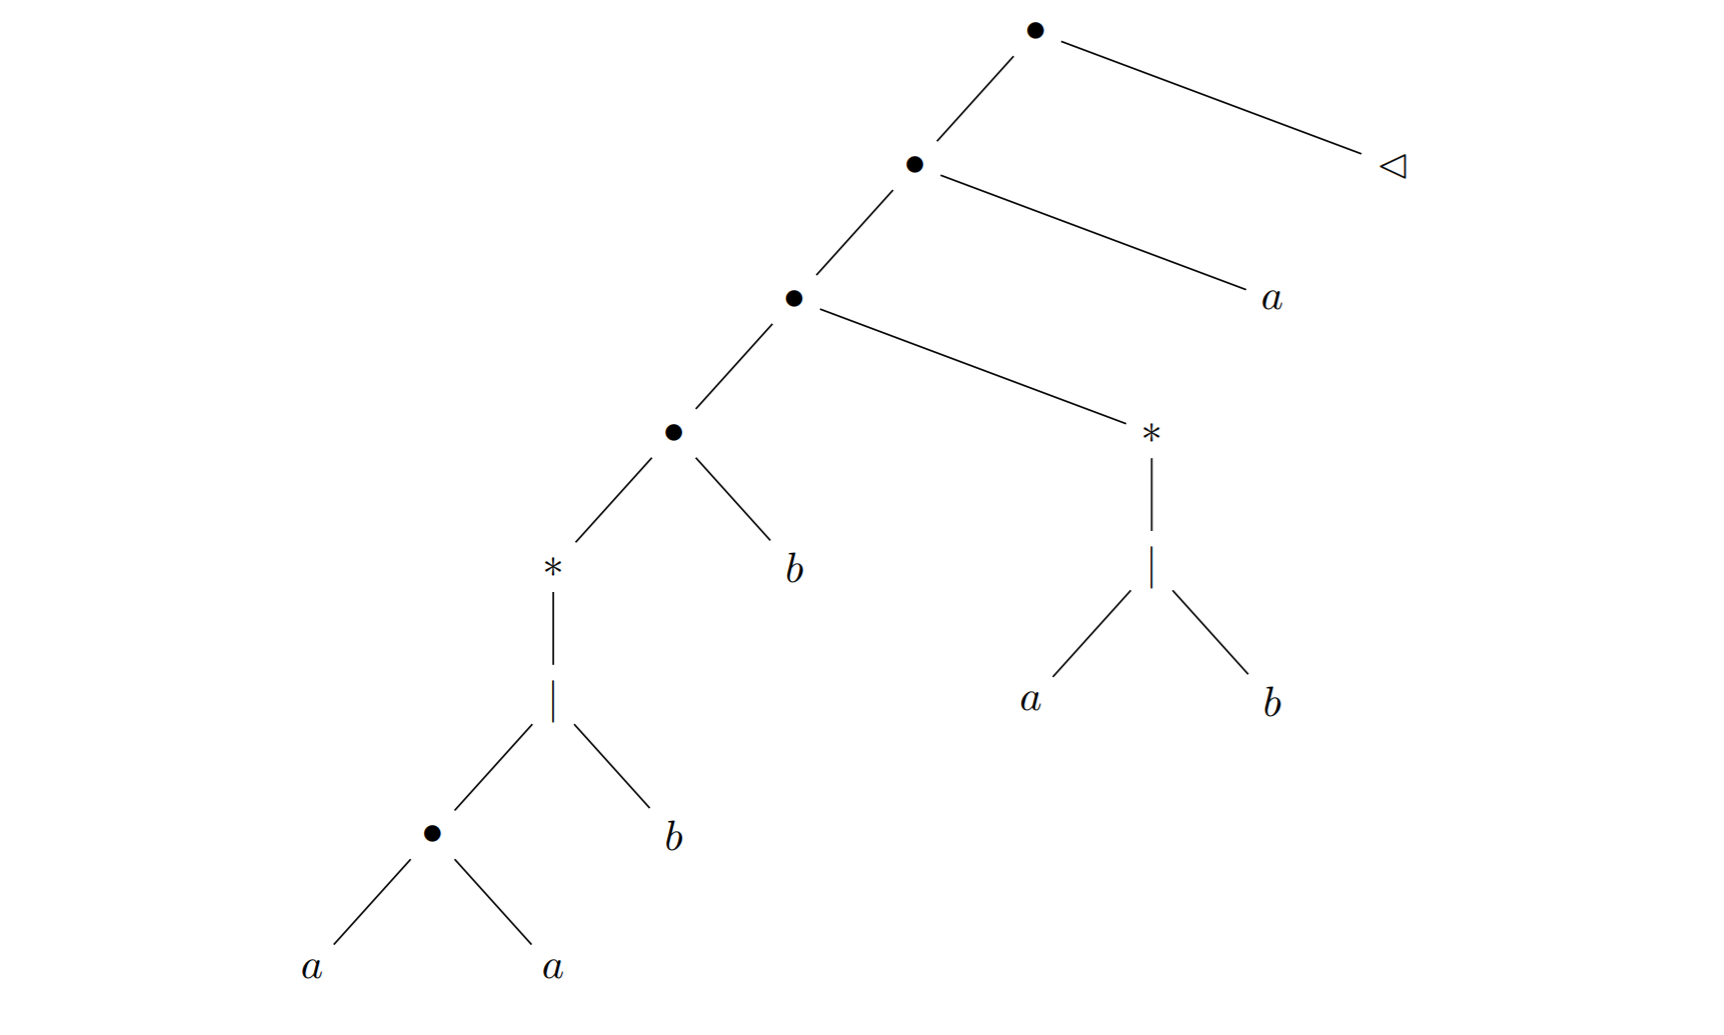
\includegraphics[width = 275px]{images/SintTree.PNG}
    \caption{Синтаксическое дерево}
    \label{fig:SyntaxTree1}
\end{figure}

Как же с помощью него вычислять функцию $FollowPos$? На самом деле одного синтаксического дерева недостаточно, нам придется ввести ещё три специальных атрибута. Пусть $u$ - узел синтаксического дерева, тогда:
\begin{Def}Символом $f_{u}$ будем обозначать значение атрибута $FirstPos(u)$ "--- множество номеров позиций, с которых может начинаться слово из $R_u$, где ($R_u$ - регулярное выражение, задаваемое вершиной $u$) \end{Def}

\begin{Def}
    Символом $l_{u}$ будем обозначать значение атрибута $LastPos(u)$ "--- множество номеров позиций, в которых может заканчиваться слово из $R_u$, где ($R_u$ - регулярное выражение, задаваемое вершиной $u$)
\end{Def}

\begin{Def}
    Атрибут $nullable(u)$ показывает содержит ли $R_u$ пустое слово ($T$ и $F$)
\end{Def}

Эти атрибуты вычисляются снизу вверх: зная атрибуты дочерних
узлов, вычисляются атрибуты родителя.
\begin{figure}[h!tp]
    \centering
    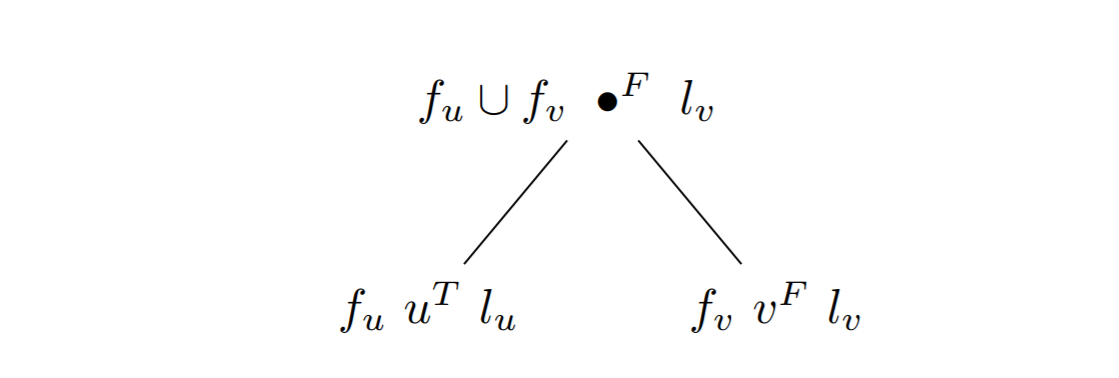
\includegraphics[width = 250px]{images/7.PNG}
    \caption{Вычисление атрибутов для одного из узлов}
    \label{fig:SampleNode}
\end{figure}

В примере на рисунке $2$ левый узел имеет атрибут $nullable$ равный $True$, а значит конкатенация (корень данного поддерева) может начинаться как с $f_u$, так и с $f_v$. С другой стороны итоговая конкатенация может заканчиваться только с $f_v$, так как правый узел имеет атрибут $nullable$ равный $False$. Атрибут $nullable$ итоговой конкатенации тоже будет равен $False$, так как мы конкатенируем слова, одно из которых точно не может оказаться пустым.


После нескольких итераций вычислений таких атрибутов мы получаем готовое синтаксическое дерево:
\newpage
\begin{figure}[h!t!p]
    \centering
    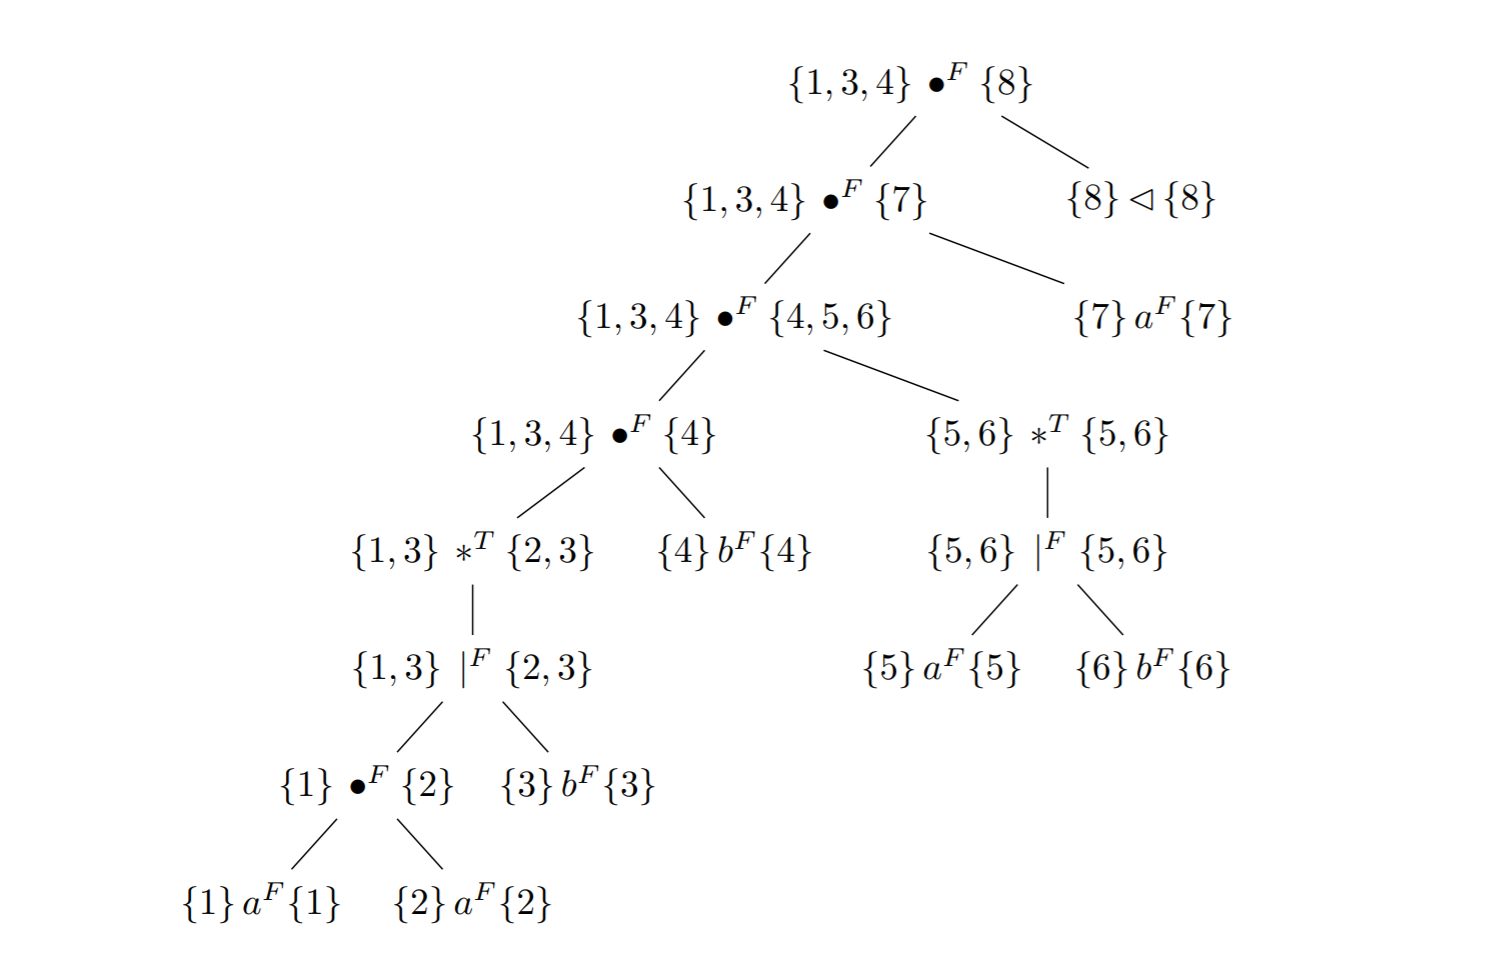
\includegraphics[width = 300px]{images/FullSintTree.PNG}
    \caption{Готовое синтаксическое дерево}
    \label{fig:SyntaxTree2}
\end{figure}


Теперь, используя рисунок \ref{fig:SyntaxTree2}, мы можем найти необходимое множество $FollowPos$ по следующему алгоритму:
\begin{enumerate}
    \item Положим сначала $FollowPos(i) = \varnothing$ для каждого номера $i$
    \item Для каждой вершины-конкатенации $u\cdot v$, для каждого $i \in LastPos(u)$ добавим к $FollowPos(i)$ множество $FirstPos(v)$.
    \item Для каждой вершины-итерации $u^{*}$, для каждого $i \in LastPos(u)$ добавим к
          \\$FollowPos(i)$  множество $FirstPos(u)$.
\end{enumerate}

Построим таблицу множества $FirstPos$ для нашего регулярного выражения:
\begin{table}[h!]
    \centering
    \begin{tabular}{c|c}
        $i$   & $FollowPos(i)$ \\ \hline
        $1_a$ & $2_a$          \\
        $2_a$ & $1_a,3_b,4_b$  \\
        $3_b$ & $1_a,3_b,4_b$  \\
        $4_b$ & $5_a,6_b,7_a$  \\
        $5_a$ & $5_a,6_b,7_a$  \\
        $6_b$ & $5_a,6_b,7_a$  \\
        $7_a$ & $8_{\lhd}$
    \end{tabular}
    \caption{множество $FirstPos$}
\end{table}

Теперь с помощью таблицы с $FirsPos$ мы можем построить следующий ДКА:
\begin{figure}[ht!p]
    \centering
    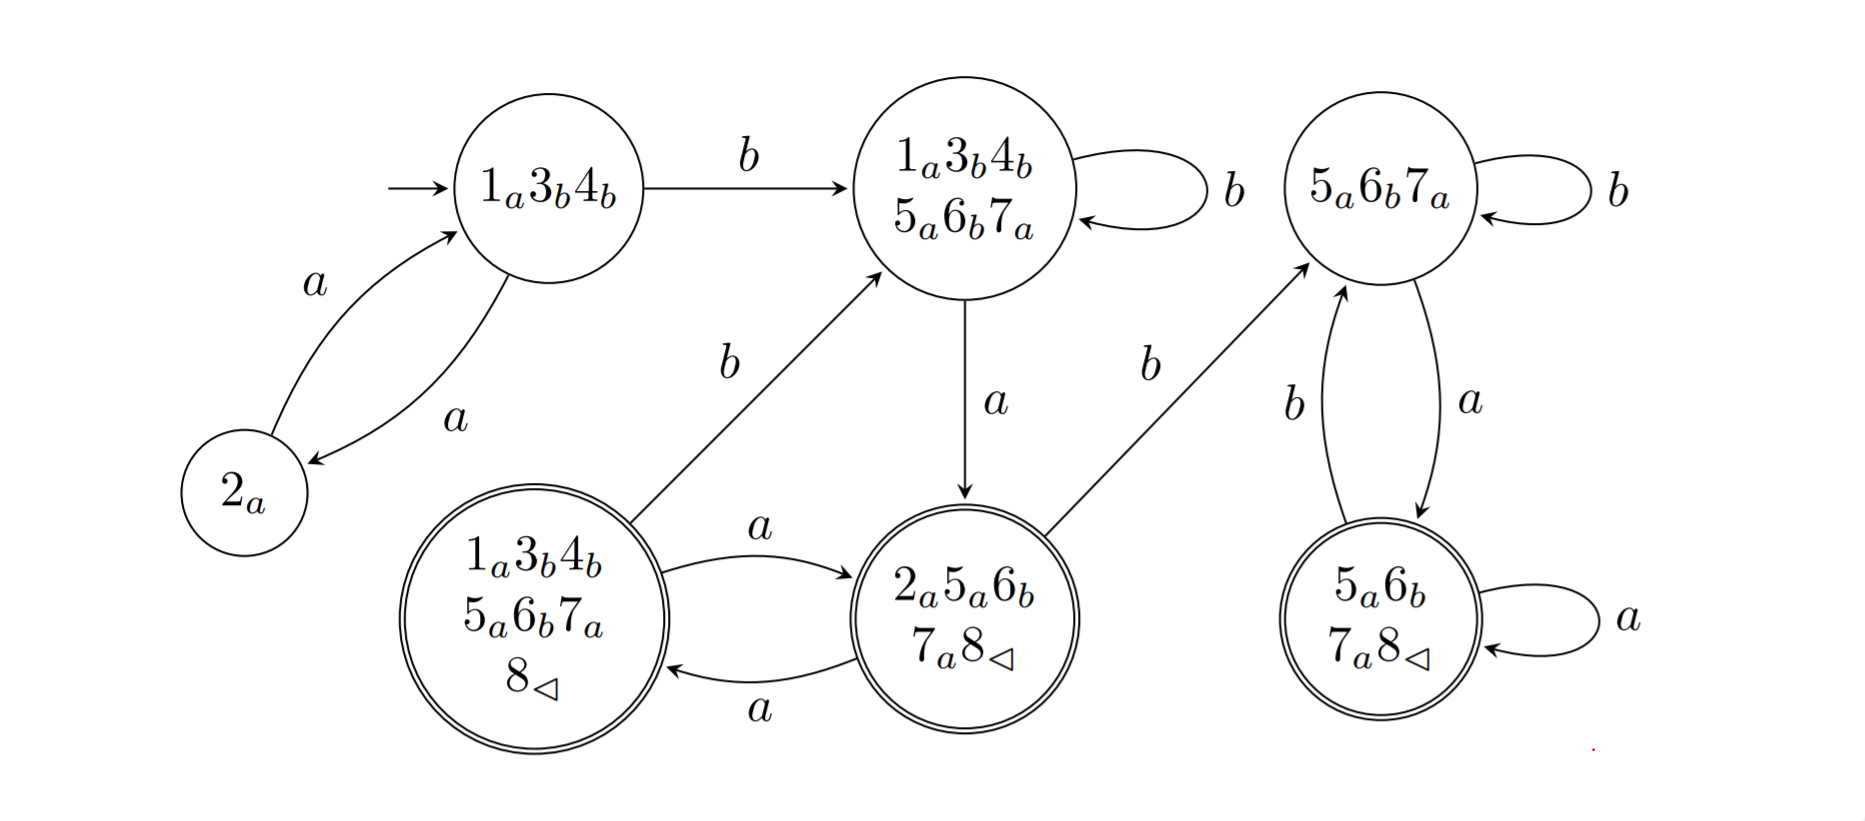
\includegraphics[width = 400px]{images/DKA.PNG}
    \caption{ДКА по таблице $FirstPos$}
    \label{fig:DFA}
\end{figure}

Начальное состояние автомата "--- это корень синтаксического дерева, поскольку атрибут $FirstPos(\text{Корень})$ как раз и будет указывать нам $FollowPos$ в самом начале. Далее проходим по таблице и строим итоговый автомат.


$\delta(S,b) = \bigcup followpos(\bigcup b)$

Проблема данного алгоритма в том, что если вы возьмете РВ и построите по нему ДКА, то оно окажется очень большим. Из-за экспоненциального роста возникают проблемы с памятью. Чтобы решить данную проблему зачастую используют НКА.

Алгоритм построения НКА мы рассмотрим на следующей лекции, а сейчас давайте построим НКА использую такой же  формализм, что и выше.

Начальное состояние - нулевая позиция. Из него будеь переход по $\varepsilon$ во все позиции, с которых слово может начинается.

Дальше для каждого отдельного символа и для каждой отдельной позиции будет просто переходы во все позиции по $followpos$. Мы уже знаем, что по символу $a$ идет переход в позицию $2a$. Из кружка, в котором написан символ позиции, идет переход во все кружки с $followpos$ от этой позиции и на переходе будет написан этот символ. Но всюду придется заменить маркер начала слова на пустое слово, и в конце добавляем новую вершину - маркер конца слова, и это состояние сделаем принимающим.

Еще раз алгоритм построения:
\begin{enumerate}
    \item Множество состояний это множество позиций
    \item Из позиции есть переход во все позиции из множества $followpos$ этот переход должен быть именно по символу из $followpos$
    \item Принимающее состояние единственное - маркер конца слова
    \item Все выходы из принимающего состояния - эпсилон переходы
\end{enumerate}


\begin{center}
    \begin{tikzpicture}[scale=0.2]
        \tikzstyle{every node}+=[inner sep=0pt]
        \draw [black] (21.1,-22.9) circle (3);
        \draw (21.1,-22.9) node {$\rhd$};
        \draw [black] (40.6,-14.5) circle (3);
        \draw (40.6,-14.5) node {$1_a$};
        \draw [black] (41.9,-26.2) circle (3);
        \draw (41.9,-26.2) node {$3_b$};
        \draw [black] (27.9,-35.9) circle (3);
        \draw (27.9,-35.9) node {$4_b$};
        \draw [black] (53.2,-14.5) circle (3);
        \draw (53.2,-14.5) node {$2_a$};
        \draw [black] (41.2,-36.6) circle (3);
        \draw (41.2,-36.6) node {$\lhd$};
        \draw [black] (41.2,-36.6) circle (2.4);

        \draw [black] (43.6,-14.5) -- (50.2,-14.5);
        \fill [black] (50.2,-14.5) -- (49.4,-14) -- (49.4,-15);
        \draw (46.9,-15) node [below] {$a$};
        \draw [black] (23.86,-21.71) -- (37.84,-15.69);
        \fill [black] (37.84,-15.69) -- (36.91,-15.54) -- (37.31,-16.46);
        \draw (31.84,-19.21) node [below] {$\varepsilon$};
        \draw [black] (24.06,-23.37) -- (38.94,-25.73);
        \fill [black] (38.94,-25.73) -- (38.23,-25.11) -- (38.07,-26.1);
        \draw (31.09,-25.15) node [below] {$\varepsilon$};
        \draw [black] (22.49,-25.56) -- (26.51,-33.24);
        \fill [black] (26.51,-33.24) -- (26.58,-32.3) -- (25.7,-32.76);
        \draw (23.82,-30.55) node [left] {$\varepsilon$};
        \draw [black] (30.9,-36.06) -- (38.2,-36.44);
        \fill [black] (38.2,-36.44) -- (37.43,-35.9) -- (37.38,-36.9);
        \draw (34.49,-36.81) node [below] {$b$};
        \draw [black] (9.9,-22.9) -- (18.1,-22.9);
        \fill [black] (18.1,-22.9) -- (17.3,-22.4) -- (17.3,-23.4);
        \draw (14,-23.4) node [below] {$start$};
    \end{tikzpicture}
\end{center}

Очевидно, регулярность будет сохраняться для любых композиций приведенных выше операций. Поэтому регулярным языком будет результат любой операции, которую можно, так сказать, "выразить в элементарных функциях". \\
Например, симметрическая разность двух регулярных языков:
$$X \triangle Y = (X \ \backslash \ Y) \cup (Y \ \backslash \ X) = (X \cup Y) \ \backslash \ (Y \cap X)$$
будет регулярным языком. \\
Разность двух регулярных языков также будет регулярна, так как
$$X \ \backslash \ Y = X \cap \overline{Y}$$

